%%%%%%%%%%%%%%%%%%%%%%%%%%%%%%%%%%%%%%%%%%%%%%%%%%%%%%%%%%%%%%%%%%%%%%%%%%%%%
\chapter{Related Work}\label{chap:authenticationandauthorization}
%%%%%%%%%%%%%%%%%%%%%%%%%%%%%%%%%%%%%%%%%%%%%%%%%%%%%%%%%%%%%%%%%%%%%%%%%%%%%

\chapterstart


"On the Internet, nobody knows you are a dog"(\cite{Steiner:Dog:1992})

The cartoon of \cite{Steiner:Dog:1992} showing two dogs sitting in front of a computer with the iconic title cited above became an illustration of how people view anonymity on the Internet. Being anonymous on the Internet, however, is not that easy anymore. The use of mobile devices has changed the way how we access information, interact with each other and share content. Digital services are used to access information, which is opening fraught opportunities to attackers who are trying to impersonate someone and access confidential information.  With this change of user behavior, the way we think of authentication and authorization methods has to adjust. Identity management is mandatory to provide a seamless user experience, including identity proofing, authentication, and assertions in federated environments [cf. (\cite{NIST:2017:DIG}), (\cite{Corre:2017:WHI})].


Users find themselves struggling using multiple devices, accounts, and services. The user's burden of this site-by-site account management is putting security at risk. The goal of new authentication and authorization solutions is to help the user managing his accounts by providing single-sign-on, based on an exchange of identity-related assertion across security domains in a scalable way [cf. (\cite{Corre:2017:WHI})].  

In this related work part existing work and methods to authenticate and authorize users a described. The part is split up in the chapters Security Considerations, Identity Proofing, Authentication, Assertion, Popular Federation Systems, Token-based Authentication and Single Sign-On.
  

\section{Security Considerations}
\label{securityConsiderations}

Before getting further into the topic of authentication and authorization, this section will shed light on some basic security principles, concerning authentication and authorization, which help to understand the need for authentication and authorization mechanisms. 

Some basic design principles formulated by \cite{Saltzer:PICS} in 1975 were paraphrased by \cite{Neumann:2018:PTC} and are still relevant today. The principles give an underlying overview of what should be the focus when designing a secure system. The first of the ten basic security principles formulated by \cite{Saltzer:PICS} is the economy of mechanism which means to keep the design as simple as possible.
The next principle describes that access should not be explicitly denied instead it should be explicitly permitted. For example, when using Access Control Lists (ACLs), all access should be explicitly denied by default. This kind of access control is called Fail-safe defaults. Furthermore, \cite{Saltzer:PICS} states the complete mediation principle, which every access to every object has to be checked for authority without exceptions. A fundamental concept that is part of these ten principles is an open design. The design of an application should not be secret. It can not be assumed that design secrecy will enhance security. This principle is applied in cryptography. The design of cryptographic algorithms is available for the public; just the keys remain secret. A broadly used principle in authentication is the separation of privileges. Separation of privileges means that two keys should be used to protect resources if feasible and privileges should be separated.  Furthermore, every application and user should be provided with lest privileges they need to complete their job. The existence of overly powerful mechanisms such as superuser is inherently dangerous - this is called least privilege. The least common mechanism principles compel to minimize the amount of mechanism common to more than one user and depended on by all users. In authentication users often get frustrated with the complicated sign-in processes. Therefore, the psychological acceptability should be kept in mind. Keep it simple. The design of the interface for the user should be easy to understand so that the user routinely and automatically applies the protection mechanism correctly. The attack factor or work factor how \cite{Saltzer:PICS} is essential to protect sensitive resources. Cost-to-protect should commensurate with threats and expected risks. It should not be possible to circumvent the mechanism with the resources of the attacker.   
The last one is a recording of compromises which means to provide trails of evidence which are tamper-proof and difficult to bypass. All of these principles are important when choosing an authentication system and need to be considered carefully. 

Besides formulating these fundamental principles which will be discussed in various forms, \cite{Saltzer:PICS} also discuss the terms "privacy" and "security". Those terms get frequently used by authors writing about information storing systems, like in this paper. However, the terms "privacy" and "security" are often used very differently. \cite{Saltzer:PICS} for example, defines "privacy" as the ability of an individual to specify whether, when and to whom sensible information is released, and "security" is described as a technique that can control who can modify resources on a computer. Another more recent description of the terms "security" and "privacy" comes form \cite{Brooks:2017:IPE}. \cite{Brooks:2017:IPE} state the importance of the distinction between privacy and security. This distinction is between privacy and security are essential because there are security issues unrelated to privacy, just as there are privacy issues that are unrelated to security. While security concerns arise from illegal system behavior, privacy concerns arise from byproducts of authorized personally identifiable information (PII) processing. Even byproducts that are considered to protect PII can raise security concerns, for example, it can be questioned to which degree a tool for persistent activity monitoring should reveal information about individuals that are related to security purposes. However, security and privacy have in common that they want to protect personal information and resources or PII [cf. (\cite{Brooks:2017:IPE}), (\cite{Saltzer:PICS})].

These security issues and privacy issues, of course, raise particular concerns for users as well as for companies offering authentication services. When it comes to protecting personal resources, there are three primary concerns. According to \cite{Todorov:2007:MUI} those three concerns are Confidentiality, Integrity, and Availability. The term confidentiality means that personal information is protected from 
disclosure to unauthorized individuals and organizations. Integrity or integrity of information is protecting information from accidental or intentional tampering. Modification of confidential data may affect the data validity. Availability is the need to be able to access information at the time a user requests it. The availability of the services that exposes information has to be given as well. In an ideal world companies offering authentication and authorization services will do everything to use the best technologies regarding countermeasures to protect confidentiality, integrity, and availability. Establishing countermeasures, however, can be costly leading to a trade-off between costs and level of production of information. A typical approach to establishing information security management is to analyze risks first and then form counter measurements [cf. (\cite{Todorov:2007:MUI})]. 

\cite{NIST:2017:DIG} splits the risk assessment into different sections, rather than combining proofing, authentication, and federation of digital services into a single Level of Assurance(LOA). In order to provide the most effective approach each of the section is analyzed regarding risk and impacts of failure. The assessment should help to avoid errors and choose based the results which technologies and mitigation strategies should be chosen. Errors that can be avoided with an extensive risk assessment are identity proofing, authentication and federation errors. Identity proofing risks include a malicious applicant successfully poses as someone else or for example the impacts of collecting more information about an applicant then required. Choosing the right level of assurance in the identity proofing process gives robustness and confidence to the determination of identity. The right authentication assurance level is chosen to mitigate problems in the authentication process, and the binding between an authenticator and a specific individual. An example of a potential error is the applicant may use credentials that not rightfully belong to them. Moreover, last but not least the accurate federation assessment helps to mitigate potential federation errors. Federation errors might occur when an identity assertion is compromised. Analyzing this risk makes it easier to choose an assurance level for each category. Therefore, the risk gets categorized of harm according to \cite{NIST:2017:DIG}: 

\begin{itemize}
	\item Inconvenience, distress, or damage to standing or reputation;
	\item Financial loss or agency liability
	\item Harm to agency programs or public interests
	\item Personal safety
	\item Civil or criminal violations
\end{itemize}

Each of the categorize can then be rated with a potential impact level which can be either low, moderate and high. The result of this risk assessment can then be the basis for choosing the appropriate identity, authentication and federation assurance level. The assurance level determination is just relevant for analyzing the risk of online transaction offered by digital services and should not be used for the complete business process which may include offline processing in a entirely segmented system. 

The result of all design principles, security and privacy considerations should be a system, network or component that is trustworthy. According to \cite{Neumann:2018:PTC} trustworthiness is given if an entity satisfies its specified requirement, after a reliable assessment. The requirements that deserve especially consideration are, those that are critical to an enterprise, mission, system, network or other entity. One of the requirements to make a system trustworthy is a reliable authentication and authorization process. These processes are discussed in more detail in the next sections.


\section{Identity Proofing}
\label{identityProofing}

“Digital identity is the unique representation of a subject engaged in an online transaction. The process used to verify a subject’s association with their real-world identity is called identity proofing” (\cite{NIST:2017:DIG})

A digital identity as explained above is the result of what is called the authentication process. It is a way of identifying the user as whom he claims to be. In order to proof the users identity presentation, validation and verification of a minimum set of attributes is necessary [cf. (\cite{Boyd:2012:GSOAuth})]. 

To become an authenticated the user has to go through certain steps on the way. These steps the user has to go through are enabled be typical components unique to the authentication process. \cite{Todorov:2007:MUI} identifies three typical components that are part of the authentication the Supplicant, the Authenticator and the Security Database. The Supplicant is the party that provides the evidence to prove the identity of a user or client. The result of the authentication process should be the authenticated user or client. The Authenticator, also called server, is responsible for ascertaining the user identity. After prove of identity, the authenticator can authorize or audit the user access to resources. Security Authority Database, which is storage or  a mechanism to check the user's credentials. The storage can be represented by as much as a flat file, a server on the network providing centralized user authentication or a distributed authentication server [cf. (\cite{Todorov:2007:MUI})]. 

\begin{figure}[h]
	\centering
	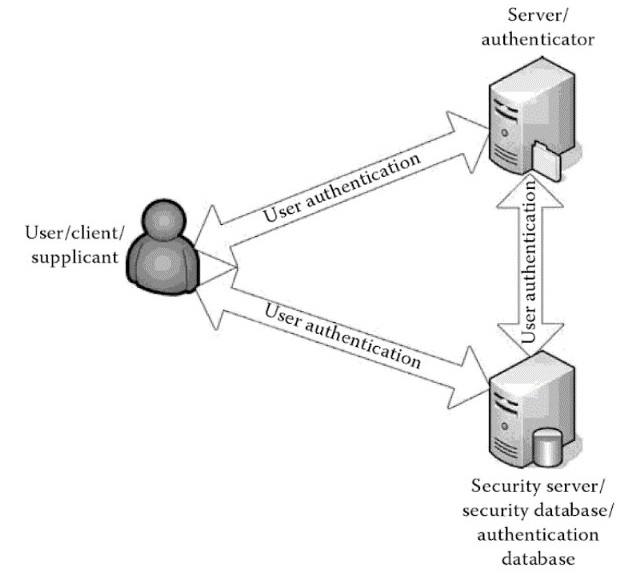
\includegraphics[width=0.8\textwidth]{images/componentsUserAuthenticationSystem}
	\caption[Componets Authentication]{Components User Authentication System}
	\label{fig:componentsuserauthenticationsystem}
\end{figure}


It is vital that all the components like shown in (figure~\ref{fig:componentsuserauthenticationsystem}), of a user authentication system can communicate independently of each other. Whether or not all communication channels are used depends on the authentication mechanism and the model of trust that it implements. For example, the Kerberos authentication protocol does not feature direct communication between the authenticator and security server [cf. (\cite{Todorov:2007:MUI})]. 

\cite{NIST:2017:DIGEIP} also describes components that are similar to the ones described by \cite{Todorov:2007:MUI} in (figure~\ref{fig:componentsuserauthenticationsystem}). Furthermore \cite{NIST:2017:DIGEIP} describes additional expectations of the identity proofing process. The expected outcome of the identity proofing process should be that the claimed identity is linked to a single, unique identity, whereas the provided evidence for the claimed identity has to be validated to proof it is correct, genuine and exists in the real world. Furthermore \cite{NIST:2017:DIGEIP} describes three different identity assurance level:

\begin{enumerate}
	\item \textbf{Identity Assurance level 1} - There is no need to link the applicant to a real-life identity. All attributes provided ar self-asserted and are neither validated nor verified.
	\item \textbf{Identity Assurance level 2} -  The evidence provided supports the real-world existence of the claimed identity. The identity proofing has to be either remote or physical-present. Attributes can be asserted by CSPs to RPs in support of pseudonymous identity with verified attributes. 
	\item \textbf{Identity Assurance level 3} - The identity proofing requires physical presence. Attributes must be verified by a authorized and trained CSP. 
\end{enumerate}
	

\section{Authentication}
\label{authentication}
For a very typical authentication process, the user provides its username and password when the application demands it. If the user provides a correct username and password, an application assumes the user is indeed the owner of the account he wants to log on. The evidence provided by the user in the authentication process is called credentials. Most of the time as mentioned above credentials get provided in the form of username and password. Nevertheless, credentials also may take other forms like PIN’s, key cards, eye scanners and so on [cf. (\cite{Todorov:2007:MUI}), (\cite{Boyd:2012:GSOAuth})]. 

Credentials, which prove the identity of an entity and find use as authenticators in authentication systems, are called factors. \cite{NIST:2017:DIG} categorize following types of factors:

\begin{itemize}  
	\item Something, the user, knows - Cognitive information the user has to remember. Examples include passwords, PIN, answers to secret questions.
	\item What the user has - something the user owns. Examples include a security token, driving license, one-time password (OTP). 
	What the user is - biometric information of the user. Examples include fingerprint, voice, and face.  
	\item What the user is - biometric information of the user. Examples include fingerprint, voice, and face. 
\end{itemize}

Other types of information which are not considered authentication factors but  can be used to enrich the authentication process according to \cite{Dasgupta:2017:AUA} are:

\begin{itemize}
	\item Where the user is - the location of the user can is used as a fourth factor of authentication. Examples include GPS, IP addresses.
	\item When the user logs on - Time can also be extracted as a separate factor. Verification of employee’s identification in different office hours can prevent many kinds of grave data breaches. The time factor can easily prevent online banking fraud events to a great extent. 
\end{itemize}

The authenticators are based on secrets that can be either public key pairs (asymmetric keys) or shared secrets (symmetric keys). Public key pairs consist of a private and a public key. The private key gets stored on the authenticator, the holder of the private key can use it to prove that he controls the authenticator. The verifier of the authenticator can then use the public key - most likely received with the help of o public key certificate - together with the authentication protocol to verify the identity of the user. Shared secrets can be either symmetric keys or memorized secrets. Both keys and passwords can be used with similar protocols. However, there is a huge difference for the user. Symmetric keys are generally stored on hardware; secrets have to be memorized by the subscriber which can lead to multiple vulnerabilities. The user chooses short, memorable passwords while cryptographic keys are typically long enough to make network-based guessing attacks untenable user-chosen passwords may be vulnerable [cf. (\cite{NIST:2017:DIG})]. 


To secure a solution properly, it should at least use two factors of the three listed above. To make use of more than one factor of a pool of potential credentials to verify the identity of a user is referred to as Multi-factor Authentication (MFA). The goal of multi-factor authentication is it to provide a layered defense and make it harder for unauthorized individuals to gain access. If one of the factors breaks, the service can still rely on the non-compromised authentication factors [cf. (\cite{Dasgupta:2017:AUA})].

Using just one factor is called Single Factor Authentication(SFA). \cite{Dasgupta:2017:AUA} clearly describes the drawbacks SFA has compared to MFA, primarily the universal used password-based authentication. The user needs to remember different passwords for multiple accounts. Therefore, the user often reuses one password also known as password fatigue.

In an Interview by \cite{Tomkins:2009:DPF} with Jon Brody, he explains Password Fatigue like the following. An average user has 15 accounts; some people might even have up to 30 accounts - far too much to manage appropriately. Users then tend to adopt specific password patterns like using simple passwords for nontransactional sites and complex passwords for banking sites. Since many complex passwords are hard to remember users also often reuse passwords for different services at one point - this is called password fatigue. 

Besides password fatigue \cite{Todorov:2007:MUI} draws attention to one of the significant challenges of secure user authentication represented by default passwords. Vendors often ship their devices with pre-configured standard passwords. Although vendors recommend changing default passwords, system architects and engineers often fail to do so because they are more focused on the business logic than on security causing security issues. Systems with default passwords are more straightforward to attack, for example by knowing or guessing the device the attacker has an easy time authenticating with the system accordingly. 


Due to the problem of password fatigue and default passwords, one factor like a password might easily get compromised. The user can then no longer use the service until the repair of the system which can lead to a delay of the user when trying to access necessary information. Also, there is a risk that the user does not notice the compromise of the single factor which can lead to devastating effects [cf. (\cite{Dasgupta:2017:AUA})]. 

When designing an authentication process by using multiple factors the designers of the process should be acutely aware of the type of application and the information that has to be secured. For example, a solution for an international bank should have different standards than an app for a making a grocery list. On the one hand, challenging and complex authentication processes for trivial applications might scare away users. On the other hand, simple methods for applications protecting sensitive data might drive users away as well. Application designers should always try to find a middle way that suits both parties, the application owners and the users [cf. (\cite{NIST:2017:DIG})]. 

\cite{NIST:2017:DIGAL} defines three different authenticator assurance levels to make sure the system a company is designing uses the appropriate authenticators for their purpose. Each of the authenticator assurance levels has to fulfill all the requirements of their successor. \cite{NIST:2017:DIGAL} describes three levels: 
\begin{enumerate}
	\item \textbf{Authenticator Assurance Level 1} - The first level states that defines that a claimant has to provide some kind of assurance that he controls an authenticator bound to subscribers account through a secure authentication protocol. The assurance can be either in the form of a single-factor or multi-factor authentication.
	\item \textbf{Authenticator Assurance Level 2} - The second level requires the use of at least two distinct authentication factors. The confidence that the claimant controls the authenticators of the subscriber's account is high at this level. Appropriated cryptographic techniques are required.  
	\item \textbf{Authenticator Assurance Level 3} - The third level of authentication provides a very high level of confidence that the claimant is in possession of the authenticators bound to the subscriber. Claimants need to prove possession of the key with two distinct authenticators through a secure authentication protocol. One of the authenticators needs to be hardware-based.
\end{enumerate}



To reflect on authentication, it can be said that authentication is a critical part of every application. As users are getting more concerned on security, the pressure on developers grows to provide a solution that secures sensible data while keeping up usability standards, which can often be a trade-off. Complex applications need complex security which can mean high costs for individually developed solutions; therefore application developers should also think about using federated authentication solutions.


\section{Assertion}
\label{assertion}
The authentication and authorization process are very closely related to each other and for users often hard to separate. After the authentication process of a user, the application has now proved that the user is whom he claims to be, but not every user is the same. After the user authenticates, the user may want to access data or services. Based on the information provided by the authentication process the application can allow or deny the user to access information or services. In other words, we have to check if the user is authorized to access data of a service. Furthermore, authorization offers granular control to distinguish between reading, write or execute access to individual resources, typically access control list (ACL) are used for each operation [cf.(\cite{Todorov:2007:MUI}, \cite{Boyed:2012:GSOA})].

Systems offer a user login process or sign-in process, in order to receive the information necessary to make authorization decisions. The login process initiates the authentication process between the user and the system. As a result of this process where the user has to prove its identity, the user receives a system or application specific structure. In a federated identity system, this is called an assertion. The assertion holds an identifier and identification information about the user which can indicate for example what kind of resources the user can access. For every action, the user then has to provide the assertion and based on the information provided within the assertion the user is then either granted or denied access. Another example of the usage of the assertion is the personalization of websites [cf. (\cite{Todorov:2007:MUI}), (\cite{NIST:2017:DIG})].

In federated systems, the verifier of authentication information of the user is called Identity Provider (IdP), and the party that receives and uses information is called the Relying Party(RP). In the context of the federated identification systems the user, or the one that is trying to access information form a system is called the subscriber. The IdP generates an assertion for the verifier associated with the subscriber. This process allows subscribers to access multiple RPs without maintaining separate credentials and the process also supports singe-sign on. \cite{NIST:2017:DIGFA}

\cite{NIST:2017:DIG} defines different levels of federation assurance that define how assertion should be constructed and secured for a given transaction. Each successive level has to fulfill the requirements of all lower level. Federation assurance levels defined by \cite{NIST:2017:DIGFA} are:

\begin{enumerate}
	\item \textbf{Federation Assurance Level 1}  - The first level requires a bearer assertion,
	signed with approved cryptography by an IdP, for example, OpenID Connect
	Basic Client profile or Security Assertion Markup Language (SAML) Web SSO
	Artifact Binding profile with no additional feature.
	
	\item \textbf{Federation Assurance Level 2} - The second level requires an assertion like the
	OpenID Connect ID Token or SAML Assertion, to be encrypted with the public
	key of the RP, whereas the RP is the only party that can decrypt the bearer
	assertion.
	
	\item \textbf{Federation Assurance Level 3} - Additionally to the first two levels the last federation assertion level requires the subscriber to prove that he is in possession of a key that is bound to the assertion (holder of key assertion) and initially was used to authenticate to the IdP. 
	
\end{enumerate}
For any assertion level, the IdP has to make sure that an RP cannot impersonate the IdP at another RP by signing the assertion. The signing of the assertion can be done by either a MAC using a shared key or a digital signature using an asymmetric key [cf. (\cite{NIST:2017:DIG}), (\cite{NIST:2017:DIGFA})].  

One of the factors that differentiates federation assurance level is the usage of assertion binding. An assertion binding can be chosen based on the RP requirements of rather the RP needs additional proof of the binding of an assertion to a particular subscriber. The two different kind of assertion binding to chose from is the bearer and holder-of-key assertions. Any party can present a bearer assertion in order to prove to have the identity of the bearer. Based on this handling of bearer assertions it can be assumed, that if an attacker is successful in capturing a bearer assertion, he can represent the subscriber that was previously associated with this bearer assertion. The attacker could present the assertion or reference to the RP and impersonate the subscriber. The holder-of-key assertion in comparison holds a reference to a key which indicates which subscriber is representing the assertion. The key is signed and asserted by the issuer of the assertion  [cf. (\cite{NIST:2017:DIGFA})].

Typically tokens are used for assertions, in this contexts tokens are software tokens which are used to provide access control for systems. The assertion binding described before can also be referred to as token profiles. Typically there are two kind of tokens that are frequently used, which is the access token and the refresh token. An access token, when it is valid can be used to access resources. If the access token is expired and not valid anymore and refresh token can be used to reclaim a new access token. OpenID Connect additionally defines an ID token which will be discussed later [cf. (\cite{Spencer:2018:APISecurity})]. 

Furthermore tokens can be passed either by reference or by value. On the one hand if a tokens are passed by reference they have to be resolved at another instance. On the other hand a token can be passed by value and already has all the necessary information about the user to establish for example a session. Those two ways of passing a token are very important when it comes to security considerations. Also token have different types. The OAuth specification for example does not specify which kind of token has to be used. \cite{Spencer:2018:APISecurity} list some of the typical tokens: 

\begin{itemize}
	\item WS-Security token (SAML)
	\item JWT tokens
	\item Legacy tokens
	\item Custom tokens
\end{itemize}

In praxis developers often use JSON Web Tokens because they are very flexible and allow to add additional claims. Also they use JSON and not XML like SAML tokens, which is much easier to process. More about JSON Tokenens can be read in the upcomming chapter Token-base Authentication [cf. (\cite{Spencer:2018:APISecurity})].

 


\section{Token-based Authentication}
\label{tokenBasedAuthentication}

The way web developers write back-end applications has changed significantly with the rising popularity of single page and mobile applications. Backend-developers no longer spend a lot of time building markup. Instead, they build APIs for front-end applications to consume. The split up of front-end and back-end allows the back-end to focus on business logic and data management while the front-end solely focus on the representation of the content. The number one way single page and mobile web applications are authenticating users according to \cite{Tkalec:2015} is token-based authentication.

\cite{Serilleja:2015:Scothio} shares the view that token-based authentication is the modern way to handle authentication. Token-based authentication should be considered because of various factors. It is optimal for mobile applications which work in a stateless way and need to adapt to the sudden change of demand in a scalable way. Furthermore, token-based authentication provides extra security and applications can pass on authenticated users to other applications. However, before taking a closer look at token-based authentication, it should be taken into account how \cite{Serilleja:2015:Scothio} and \cite{Tkalec:2015} concluded that token-based authentication is the best alternative for modern web applications to authenticate their users. Therefore, \cite{Serilleja:2015:Scothio}, for example, examines how authentication was done in the past. One approach to authenticate users used in the past that puts token-based authentication in perspective is server-based authentication. 

\subsection{Server-Based Authentication.}
A lot of modern-day API’s built on the Representational State Transfer(REST) programming paradigm which basis is the HTTP protocol which is stateless as well. A protocol that is stateless does not recall the actions that were taken beforehand which mean for example that if we authenticate the user, in the next request we have to authenticate the user again because the application will not know the user anymore [cf. (\cite{Serilleja:2015:Scothio})]. 

The aim of server-based authentication is for the application to remember the user that logged on at the application. The application has to store the information on the server, which can be done in a few different ways on the session, usually in memory on the disk. The workflow of a server-based authentication starts with the server delivering the website and the user logging in with username and password. The server saves the information from the user login info in a session. After the session is established, the session is checked on the server for every request. If the session is valid, the server returns the requested data to the server. However, since modern single-application ant mobile applications are on the rise, this method to authenticate user shown some problems, especially when it comes to scalability [cf. (\cite{Serilleja:2015:Scothio})]. 

The session handling with server-based authentication is especially hard on the server’s bandwidth. Most of the time the session gets established in memory on the server when the user authenticates. This approach leads to an enormous overhead. The second problem with this approach is that the information of the user is held in memory on the server. Since more and more companies are moving servers to the cloud, this is not only a security issue but replicating servers to scale is limited. Also nowadays users want to access their data at any moment from every device. Providing the user with the possibility to access data across multiple mobile devices is vital, which means cross-origin resource sharing has to be enabled. With server-based authentication, it is possible to run into problems with the forbidden request when the user tries to access data from another domain [cf. (\cite{Serilleja:2015:Scothio})].


\subsection{
	Token-based authentication with JSON Web Token
}

The most important thing about token-based authentication is that it is stateless, much like HTTP. The server does not have to hold the session of the user over an extended period on the server. Instead, the user can request resources by offering a token generated by an authentication server. The token send in the query string or Authorization header can then be validated at the resource server, and the secure resource will be returned to the user. The approach of using JSON Web Tokens gives one the ability to scale applications without considering on which domain the user logged on. Another advantage besides being scalable is that token-based authentication gives one the possibility to reuse the same token for authenticating the user. Therefore, it gets easier to build applications that share permission with other application because many separate servers, running on multiple platforms and domains can reuse the same token. The approach also gives performance advantages compared to server-side authentication because there is no need to find and deserialize the session on each request. However, since it is best practice to encrypt the token, the token still needs to be validated, and the content needs to be parsed. One way to implement token-based authentication is with the help of JSON Web Tokens. JSON Web Tokens are gaining popularity fast and are backed by huge companies like Google and Microsoft. Also, the Internet Engineering Task Force defines a standard specification. OpenID and OAuth also use the JSON Web Token as a standard; therefore, the usage of the JSON Web Token will be explained in detail [cf. (\cite{Tkalec:2015})].


JSON Web Token (JWT) is a compact structure that holds information about the authentication of a user or claims. The structure is indented for space-constrained environments such as HTTP Authorization headers. The payload of the JSON Web Token is of JSON, enabling the claims to be digitally signed or integrity protected with a Message Authentication Code (MAC) and encrypted [cf. (\cite{JWT:IETF:Jones:2015})].

The standard is used to transport data between interested parties. The transferred data can be for example the identity of a user or user’s entitlements. Furthermore, with the possibility of digital signatures and encryption data can be transferred securely over an unsecured channel. The signatures also allow asserting the identity of a user if the recipient trusts JWT is asserting party [cf. (\cite{Siriwardena:JWTJWSJWE:2016})].

An example of a JWT Token is an id\_token. Google provides for Developers an OAuth 2.0 Playground, where developers can choose a scope and try it out against the Google API. To get an excellent example of a JWT, OAuth2 API v2 was selected and authorized the API [cf. (\cite{Google:2018:OAuthPlayground})].


\begin{figure}[h]
	\centering
	
\includegraphics[width=0.8\linewidth]{images/googleOAuthPlaygroundOAuthAPI}
	\caption[OAuth API]{Google Developers Playground OAuth 2.0 API}
	\label{fig:googleoauthplaygroundoauthapi}
\end{figure}

After choosing and authorizing, the API Google returns an Authorization Code. This Authorization Code is specific for a certain Authentication Flow defined by OAuth and can then be exchanged for the tokens. As a result, all information for the scopes that were selected beforehand is returned. Because OAuth 2 API v2 was selected, the returned value is an id\_token. This id\_token is a nice representation of a JWT and holds the standard information that is required according to the OAuth specification  [cf. (\cite{Google:2018:OAuthPlayground})].


\lstset{caption=JWT Token,breaklines=true, breakatwhitespace=true, basicstyle=\small\ttfamily, label={lst:jwt}, tabsize=3, basewidth={0.55em}, fontadjust, language=XML}

\begin{lstlisting}
eyJhbGciOiJSUzI1NiIsImtpZCI6ImRhZDQ0NzM5NTc2NDg1ZWMzMGQyMjg4NDJlNzNh
Y2UwYmMzNjdiYzQifQ
.
eyJhenAiOiI0MDc0MDg3MTgxOTIuYXBwcy5nb29nbGV1c2VyY29udGVudC5jb20iLCJh
dWQiOiI0MDc0MDg3MTgxOTIuYXBwcy5nb29nbGV1c2VyY29udGVudC5jb20iLCJzdWIi
OiIxMTIzMDE5MzgzMjI4MTAyMzk3MTIiLCJlbWFpbCI6ImNvcm5lbGlhcmF1Y2hAZ214
LmF0IiwiZW1haWxfdmVyaWZpZWQiOnRydWUsImF0X2hhc2giOiJSdjJRQjZoZzFqdDZR
aHRJWG5laWVnIiwiZXhwIjoxNTI5NzQ3MTk2LCJpc3MiOiJodHRwczovL2FjY291bnRz
Lmdvb2dsZS5jb20iLCJpYXQiOjE1Mjk3NDM1OTYsIm5hbWUiOiJDb25ueSBSYXVjaCIs
InBpY3R1cmUiOiJodHRwczovL2xoNC5nb29nbGV1c2VyY29udGVudC5jb20vLWJFbEt3
aDVaNUJnL0FBQUFBQUFBQUFJL0FBQUFBQUFBQk5rL0p5Qm1XTW9uYUlJL3M5Ni1jL3Bo
b3RvLmpwZyIsImdpdmVuX25hbWUiOiJDb25ueSIsImZhbWlseV9uYW1lIjoiUmF1Y2gi
LCJsb2NhbGUiOiJkZSJ9
.
yibOtrXy9_-cfOWytzwGuE4zqLv-MK_2-PYIKR_xecJt9ACnMnNMSmio6i8Vu7U061wF
OTb-qRennHbvy3lTRZLcTXttIrIUl-NdnZs2BrTSGWrw9aRzEjIHAXiY4fGRHj9VZXs_
_J3Nn0EoBmT7Cnua2hb4U_X3hAyGpEvlSGKc5HvbyzOAtNh081Cyj1TI-AidCPTuC5vh
68C55tLJ87PWNm8WU1rCPOPBdVTjhYlqJKCpgUJ39_p_MXL_uHBZXRrvbOyV_tZVlw47
rjd8GFnBq1QqsYAR-6wrFbNL1pY6tPyriqZnQdi5KqYWPUwGpXbFDUfhZAmWXT8-PTsc
gQETEp8o3RvRHtfSu8Gx4UOhukt9_VxVdHmpFw
\end{lstlisting}


The JWT Token in the figure above is presented as a sequence of URL-save base64url-encoded values. The different values are separated by a (‘.’) character. How many parts a JWT has is dependent on how the JWT is serialized. Either by using the JWS Compact Serialization or JWE Compact Serialization  [cf. (\cite{JWT:IETF:Jones:2015})].


To make sense of this JWT token in the figure above it is best to look at each of the three parts of the JWT separately. When decoding the first part of the JWT, we receive a JSON object. Each part can be decoded individually but if a quick representation of a token is needed developers are the best advised to use \href{https://jwt.io/} {https://jwt.io/}. The website not only decodes the information of the token it also verifies the token. The figure above shows a warning that pops up if the token is not flawless. The verification of the token and the signing is done with multiple libraries that inform about certain vulnerabilities of the JSON Web Token. The first decoded part of the JWT gives us the following JSON.


\lstset{
	caption=JOSE Header,
	label={lst:joseheader},
	string=[s]{"}{"},
	stringstyle=\color{blue},
	comment=[l]{:},
	commentstyle=\color{black}
}
\begin{lstlisting}
{
"alg": "HS256",
"typ": "JWT"
}
\end{lstlisting}


The JSON object in \ref{lst:joseheader} is the JOSE Header, representing the type of the token, the cryptographic operations applied and optionally additional properties of the JWT. Based on the information of the JOSE Header it can explain if the JWT is a JWS or a JWE. When speaking of JWT, we speak of one of the implementations of JWT because in fact, JWT does not exist itself. Concrete implementation of the JWT is JSON Web Signature (JWS) or JSON Web (Encryption). The figure below gives an optical representation of the structure [cf. (\cite{Siriwardena:JWTJWSJWE:2016})].

\begin{figure}[h]
	\centering
	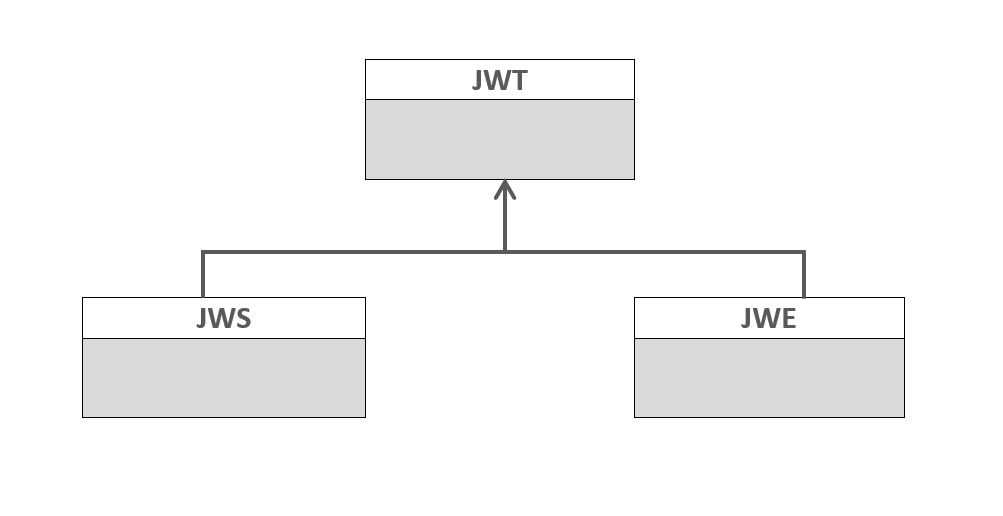
\includegraphics[width=0.8\linewidth]{images/jwtjwsjwe2}
	\caption{JWT Inheritance}
	\label{fig:jwtjwsjwe2}
\end{figure}


The 'type' Header Parameter we can examine in \ref{lst:joseheader} indicates the kind of token, considering the example it is a JSON Web Token. The second parameter is the 'alg' Header Parameter and is specified in either the 'JSON Web Security (JWS)' reference documentation written by \cite{JWS:IETF:Jones:2015} or the JSON Web Encryption (JWE) reference documentation written by \cite{JWE:IETF:Jones:2015}. In this case, the JWT is a JWS since a JWE needs more specific Header Parameter. In the JWS the 'alg' Header Parameter gives information about the algorithm which was used to create the signature. Which kind of arguments are accepted by the 'alg' Header Parameter are explained in yet another specification called 'JSON Web Signature and Encryption Algorithms' written by \cite{JWA:Jones:2015}. In the example \ref{lst:joseheader} the 'HS256' algorithm is used, meaning that the JWS was MACed using the HMAC SHA-256 algorithm. The definition of the 'alg' Header Parameter in the 'JSON Web Signature (JWS)' reference documentation is very similar to the definition in the 'JSON Web Encryption (JWE)' reference documentation except the cryptographic algorithm is used to encrypt or determine the value of the CEK. \cite{JWE:IETF:Jones:2015} also defines an 'enc' Encryption Algorithm Header, which is used for content encryption on plaintext. The authenticated encryption performed produces a ciphertext and the authentication tag. Also for the 'enc' Header Parameter, the valid arguments can be found in the 'JSON Web Signature and Encryption Algorithms' written by \cite{JWA:Jones:2015}. The algorithm used must be an AEAD algorithm with a specified key length. There is further Header Parameter that can be defined, here are just the most essential JOSE Header Parameter for this document listed. 

The second decoded part of the example in \ref{lst:jwt} JWT Token, represents the claim set. The representation of the claim set is a JSON, where each key has to be unique. If the keys are duplicated one can either end up with a JSON parsing error or the last one of the duplicated keys is returned. 

\lstset{
	caption=Claim Set,
	label={lst:claimset},
	string=[s]{"}{"},
	stringstyle=\color{blue},
	comment=[l]{:},
	commentstyle=\color{black}
}
\begin{lstlisting}
{
"azp": "407408718192.apps.googleusercontent.com",
"aud": "407408718192.apps.googleusercontent.com",
"sub": "112301938322810239712",
"email": "corneliarauch@gmx.at",
"email_verified": true,
"at_hash": "Rv2QB6hg1jt6QhtIXneieg",
"exp": 1529747196,
"iss": "https://accounts.google.com",
"iat": 1529743596,
"name": "Conny Rauch",
"picture": "https://lh4.googleusercontent.com/-bElKwh5Z5Bg/
AAAAAAAAAAI/AAAAAAAABNk/JyBmWMonaII/s96-c/photo.jpg",
"given_name": "Conny",
"family_name": "Rauch",
"locale": "de"
}
\end{lstlisting}

The decoded value form the example in Listing \ref{lst:jwt} of the Google OAuth 2.0 Playground \cite{Google:2018:OAuthPlayground} returns a JSON object shown in the Listing \ref{lst:claimset}. The claim set we receive is composed of mandatory and optional claims. Specifically requested in this example were the login, email and profile scope which affected the claims returned from the Google OAuth 2.0 API. Mandatory claims for the login with OpenID are iss, iat, aud, sub and exp and an optional clam that was returned from the API is azp. This claims will be discussed in more detail in the chapter on OpenID and OAuth 2.0. For the profile scope, the specific claims that were returned are name, picture, given\_name, family\_name, and locale. Email specific claims are email and email\_verified. Furthermore, identity providers can include additional elements that are neither mandatory or optional claims [cf. ({\cite{Google:2018:OAuthPlayground}),(\cite{Siriwardena:JWTJWSJWE:2016})]}].

The last and third part from the example in  Listing \ref{lst:jwt}  represents the base64url-encoded signature. To know which kind of signature the decoded code is resembling a peek at the JOSE Header will help. The JOSE Header as mentioned before gives information about the cryptographic elements that were used related to the signature. In case of Listing \ref{lst:signaturejwt} the Google OAuth 2.0 API uses RASSSA-PKCS1-V1\_5 with the SHA-256 hashing algorithm. However the \href{https://jwt.io/} {https://jwt.io/} website does not provide us with the decoded public key. 

\lstset{
	caption=Signature JWT,
	label={lst:signaturejwt},
	string=[s]{"}{"},
	stringstyle=\color{blue},
	comment=[l]{:},
	commentstyle=\color{black}
}
\begin{lstlisting}
{
RSASHA256(
base64UrlEncode(header) + "." +
base64UrlEncode(payload),
Public Key or Certificate.
)
}
\end{lstlisting}


To serialize an encrypted message, one has to follow either the JWS or the JWE specification. Each of the specifications has the type’s compact serialization and serialization. Google OpenID Connect uses the compact serialization. In fact, the OpenID Connect specification suggest using the JWS compact serialization or the JWE compact serialization. In this paper only the compact serialization will be discussed, the specification of the other serialization method can be either looked up in the JWE specification or the JWS specification. To call a JWS or a JWE, a JWT it has to follow the compact serialization [cf. (\cite{JWS:IETF:Jones:2015}), ({\cite{JWE:IETF:Jones:2015})].
	
	The aim of the JWS Compact Serialization is it to present content as a compact, URL-safe string, which is either digitally signed or MACed. It is not possible to use multiple signature or MAC in a JWS Compact Serialization and furthermore it is not allowed to use JWS Unprotected Headers. An unprotected header is a JSON object which includes the header element that is not integrity protected, which concludes that a protected header is a JSON object that is integrity protected by using MAC or digital signatures. A JWS Compact Serializations is represented as a concatenated string [cf. (\cite{JWS:IETF:Jones:2015})].
	
	\lstset{
		caption=JWS Compact Serialization,
		label={lst:jwscompactserialization},
		string=[s]{"}{"},
		stringstyle=\color{blue},
		comment=[l]{:},
		commentstyle=\color{black}
	}
	\begin{lstlisting}
	{
	BASE64URL(UTF8(JWS Protected Header)) '.'
	BASE64URL(JWS Payload) '.'
	BASE64URL(JWS Signature)
	}
	\end{lstlisting}
	
	The first element is called the JOSE header which contains all the information that advertises the public key corresponding to the private key that was used to sign the message. Elements of the header include the jku, jwk, kid, x5u, x5c, x5t and x5t\#s256. The second element is the JWS Payload or the content to be signed, which does not have to be JSON. To construct the message the following approach is used  ASCII(BASE64URL-ENCODE(UTF8(JOSE Header)) '.' BASE64URL-ENCODE(JWS Payload)). 
	The last element is the JWS signature, which is computed over the message that was constructed beforehand, using the algorithm defined in the JOSE Header. These three key components together are called a JWS token. When using the JWE Compact Serialization, the output is called JWE token. Compared to the JWS token, which we saw above the JWS token consists of 5 different key components [cf. (\cite{JWS:IETF:Jones:2015}), (\cite{JWE:IETF:Jones:2015})].
	
	
	\lstset{
		caption=JWE Compact Serialization,
		label={lst:jwecompactserialization},
		string=[s]{"}{"},
		stringstyle=\color{blue},
		comment=[l]{:},
		commentstyle=\color{black}
	}
	\begin{lstlisting}
	{
	BASE64URL-ENCODE(UTF8(JWE Protected Header)) '.'
	BASE64URL-ENCODE(JWE Encrypted Key) '.'
	BASE64URL-ENCODE(JWE Initialization Vector) '.'
	BASE64URL-ENCODE(JWE Ciphertext) '.'
	BASE64URL-ENCODE(JWE Authentication Tag)
	}
	\end{lstlisting}
	
	Both digital signatures and MACs can be used to provide integrity checking. However, specification warns that there significant differences that have to be considered when designing a protocol. MACs only provide the origination of the identification under specific circumstances. It is normally assumed that the private key used for the signature is only known by a single entity. Although in the case of MAC keys all the entities that use it for integrity computation need to know the MAC key in order to validate the message. That means that with MAC validation one can tell if a message is generated from one of the entities that know the symmetric MAC key and not where the message originated [cf. (\cite{JWT:IETF:Jones:2015})].	
	
\section{Single Sign-On Federation Systems}

Application security is a complex task and developing a customized siloed identity solution can be expensive. A Stand-alone identity store can besides being expensive also causes information assurance and administrative problems for organizations  [cf.(\cite{JerichoSystems:IS})]. 

A federate authentication or identity federation says \cite{Boyed:2012:GSOA} is a system that is maintaining its accounts, for example, username and password databases, with the help of third-party service. Often big cooperate IT environments already use such solutions. Environment applications, for example, may trust an Active Directory server, an LDAP server or a SAML provider [cf. (\cite{Birell:2013:FIMS}), {\cite{Boyed:2012:GSOA}].
	
	
	As shown in (figure~\ref{fig:federation}) an identity system usually consists of three parties. The user/subscriber, service provider/resource provider, and the identity provider. Depending on the protocol which is used, different information passes between the three components at different times. While the user/subscriber communicates with the IdP and the RP over a browser the IDP and the RP can communicate over a front channel which works through redirects involving the subscriber or a back channel which is a direct connection not including the subscriber [cf. (\cite{NIST:2017:DIGFA})]. 
	\begin{figure}[h]
		\centering
		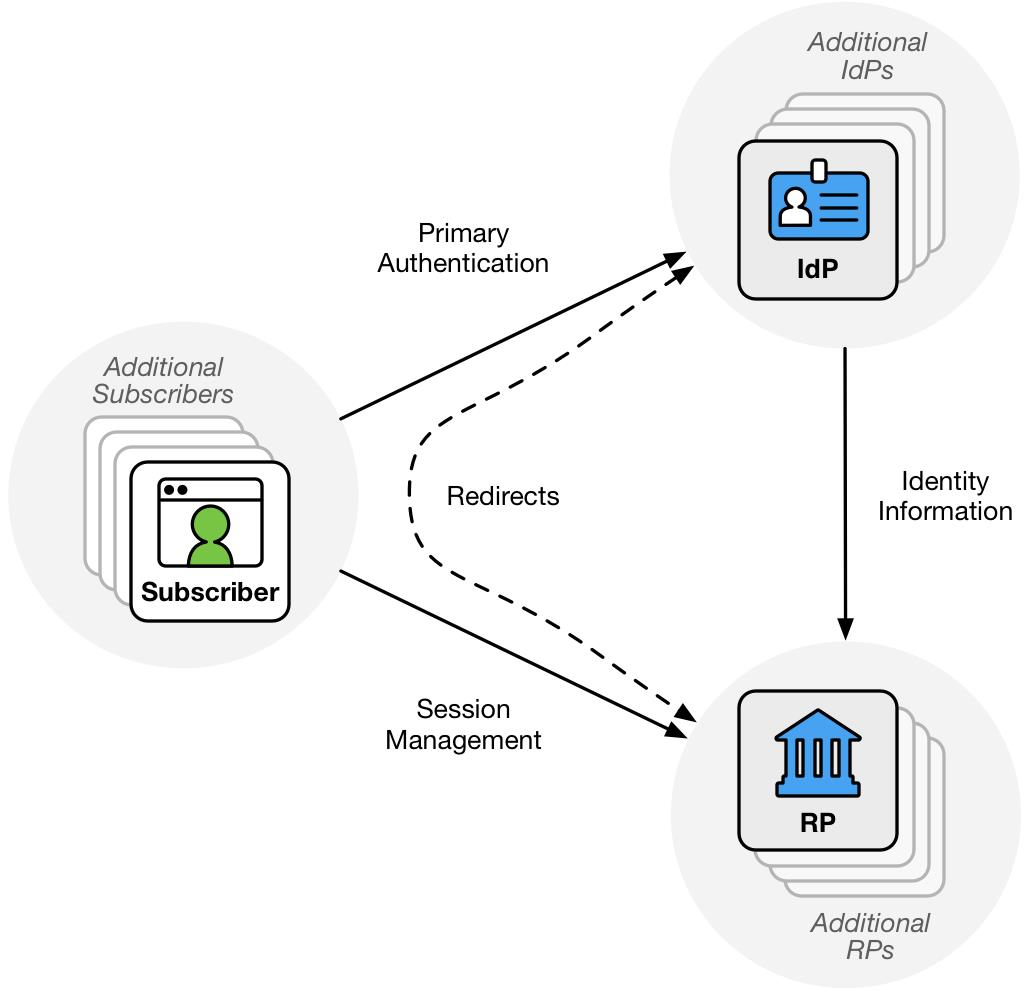
\includegraphics[width=0.8\textwidth]{images/federation}
		\caption[Federation]{Federation}
		\label{fig:federation}
	\end{figure}
	
	
	The user/subscriber is usually associated with a real user, and its identity is represented by a set of attributes. Single user can be associated with multiple identities. A service/resource provider is responsible for making an authorization decision based on authentication assertion and the attributes derived from it. Many of the service providers implement their identity management, but in federate systems, the identity management is outsourced to the identity provider. An identity provider can be either a stand-alone service or be a part of the service provider. The responsibility of the IdP is it to authenticate the user, issuing authentication assertions, manage identities whereas the IdP has the right to create, update, release and delete attributes associated with the identity [cf. (\cite{Birell:2013:FIMS})]. 
	
	
	\cite{NIST:2017:DIG} claims that identity federation is preferred over some siloed identity solution that each serve a single agency or Relying Party (RPs). Furthermore \cite{NIST:2017:DIG} lists specific benefits that come with using federated architectures, as can be examined before. 
	
	\begin{itemize}
		\item Enhanced user experience. For example, an individual can be identity proofed once and reuse the issued credential at multiple RPs. 
		\item Cost reduction to both the user (reduction in authenticators) and the agency (reduction in information technology infrastructure). 
		\item Data minimization as agencies does not need to pay for collection, storage, disposal, and compliance activities related to storing personal information. 
		\item Pseudonymous attribute assertions as agencies can request a minimized set of attributes, to include claims, to fulfill service delivery. 
		\item Mission enablement as agencies can focus on the mission, rather than the business of identity management.
	\end{itemize}

 Essentially switching to a federated identity solution should help to reduce the management burden that comes from managing multiple accounts and can lead to potential points of failure.  Furthermore users are giving control over there attributes' dissemination which leads to privacy violations and identity theft. Most of the existing identity federation solution focuses on individual system, each of which focuses on one of three general types of functionality - single sign-on, federated identity or anonymous credentials. Single sign-on system have the possibility to issue authentication assertion to multiple service providers. Examples for single-sign on are Passport, OpenID or Shibboleth. Federated identity systems are focused on managing multiple identities for a single user. Example for Federated identity are Project Liberty (http://projectliberty.org), Higgins (www.eclipse.org/higgins), PRIME (www.prime-project.eu), CardSpace, and
Client-Side Federation. Anonymous credentials systems provide authentication assertions while not revealing the user's identity to a service provider. Examples include Idemix, U-Prove, and P-IMS [cf. (\cite{Birell:2013:FIMS}), {\cite{Boyed:2012:GSOA}].
	
	\subsection{Singel Sign-On}	The focus of this thesis is on mobile SSO solutions. Therefore only SSO solution will be discussed. The aim of SSO is to design an authentication system that serves the interests of the user as well as the interests of the service provider. Whereas the user prefers a simple process, the service provider requires a complicated authentication procedure. Ironically trying to make the authentication procedure more save often leads to weakening the whole system due to the user always finding new ways to bypass it. An example mentioned before is password fatigue. Another challenge that SSO is trying to tackle is that standard web authentication solutions that require the user to login with a password, only authenticate the user and are not capable of providing access control or revealing additional information about the user. Most SSO solutions, therefore, try to combine the authentication process and authorization [cf. (\cite{Prochazka:2010:UCA})].
	
	The paper Taxonomy of Single Sign-On System \cite{Pashalidis:2003:10.1007/3-540-45067-X_22} identifies four generic architectures for SSO systems. An SSO system has to authenticate a user to a SP. Because authentication also implies identification, SSO systems have to incorporate the lifecycle management of identifiers that can take various forms. The paper distinguishes between two main types of SSO systems. The first type is ‘pseudo-SSO’ and the second type is ‘true SSO’. Typical pseudo-SSO are providing automatic authentication for all SP specific authentication methods after the user initially authenticated with the pseudo-SSO component, which is called primary authentication. The responsibility of a pseudo-SSO service is to manage all identities. A user may have multiple SSO identities for a single SP, but in principle, one SSO identity corresponds to one SP. Compared to the pseudo-SSO system in a true-SSO system, the user has to initially authenticate with the Authentication Service Provider (ASP) that is required to have an established relationship with all SPs. The relationship between the ASP and the SP has to be trustworthy. A key functionality of the true-SSO service is that the only authentication that includes the user occurs between the user and the ASP. The SP will get notified of the authentication status, including information about the identity of the user, with so-called authentication assertions. The categorization of SSO architectures can be further distinguished by the location of the ASP/pseudo-SSO component. This component can be either local to the user platform or offered as a third-party service also called SSO-proxy. This further categorization leads \cite{Pashalidis:2003:10.1007/3-540-45067-X_22} to the four generic architectures mentioned above Local pseudo-SSO systems, Proxy-based pseudo-SSO systems, Local true SSO systems and Proxy-based true SSO systems.
	
	When opting for a particular SSO architecture, one has to consider the strength and weaknesses of each system carefully. The paper, therefore, analyses the four generic architectures regarding Pseudonymity and Unlinkability, Anonymous Network Access, Support for User Mobility, Deployment Costs, Maintenance Costs, Running Cost and Trust Relationships. Pseudonymity and Unlinkability refer to the fact that the user providers sensible information that needs to be protected and it should not be possible to correlate distinct identities of the same user and personal information, and potential properties should not be linked to the user. The unlinkability cannot be guaranteed for pseudo-SSO because the identities for the SSO are SP specific. To improve unlinkability   \cite{Pashalidis:2003:10.1007/3-540-45067-X_22} suggest to use an ‘anonymizing proxy’, for local SSO system additionally services are needed for proxy-based SSP it can be integrated. User mobility is supported for proxy-based SSO, for locale SSO there needs to be further services in place. The deployment cost is lower for pseudo-SSO systems then for true-SSO systems. However, the maintenance cost is higher because if any SPs change the whole logic of the pseudo-SSO system has to change. The running cost of pseudo-SSO is likely to be lower than for true-SSO systems. For the pseudo-SSO systems, the trust relationship between users and SP may be dynamically changing depending on the implementation, for true-SSO the trust relationship is established between ASP and SPs and is always consistent. Generally speaking are pseudo-SSO systems more suitable for a closed system where identity management is just for managing the life cycle of remaining credentials. For an open system maintaining credentials is not enough. Appropriate privacy protection services and privacy-aware Identity Management schemes should be therefore integrated with true SSO schemes [cf. (\cite{Pashalidis:2003:10.1007/3-540-45067-X_22})]. 
	
	
	
	 therefore two very popular assertion technologies are discussed: Shibboleth (SAML) and OpenID Connect. Those technologies are not all possible single sign-on assertion technologies. However, they present the most commonly used in federated identity systems. According to \cite{Lynch:2017:IIG} two SSO solutions gained broad acceptance. On the one hand, SAML-based federations using SOAP, focusing on large enterprises also including governments and educational networks. On the other hand, the Web Authorization Protocol was introduced which is a combination of the Protocols OpenID and OAuth. SAML federations have been customized to address the security concerns of those institutions that typically have a large user base, significantly protected resources, complex authorization patterns and data and services spread across multiple domains. However, in a Web 2.0 world, the SAML solutions where seen as too rigid and too severe to maintain; a lightweight SSO was needed, therefore the Web Authorization Protocol was designed. The approach of this protocol is taking advantage of the lightweight RESTful APIs which are reusing the existing HTTP architecture features and the JavaScript Object Notation(JSON).
	
	
		
	\paragraph{SAML}
	\label{SAML}
	One of the well-known solutions based on Security Assertion Markup Language version 2 (SAML2) is Shibboleth. Shibboleth is one of the leading middlewares for building identity federations in a higher education sphere. To offer authentication, authorization and attribute assertion between entities. \cite{Prochazka:2010:UCA} identifies the following entities defined by Shibboleth are Identity Provider (IdP), Service Provider (SP), Discovery Service, Metadata Operator and Federation Operator.
	
	The discovery service is used to find the users organization IdP. The IdP defines an attribute release policy and releases different sets of the user's attributes to different SPs. Users are only able to agree or disagree with the whole set of attributes because the decision comes from the IdP. When the user tries to log on, to a service of a Service Provider, he gets redirected to a page where he can choose and IdP previously found by the Discovery Service. If an SP wants to provide its service to multiple federations it has to negotiate policy and technical detail with each federation operator. The federation operator manages the federation policies and introduces SPs and IdPs. Furthermore, the federations operator has to maintain and manage the information about all entities in a federation which is contained in the Metadata. A problem with this architecture is that the SP has to keep track of changes of the technical specification of various federation operators to maintain the configuration for each federation operator. A solution would be a significant federation registration, but this is indeed not possible because of technical and administrative severity and political will. This solution is also somewhat misleading for users since they have to maintain multiple credentials, select from multiple identifiers and so on [cf.\cite{Prochazka:2010:UCA}].
	
	According to \cite{Prochazka:2010:UCA} Shibboleth is too restrictive, a solution with a centrally managed point of IdPs and SPs is preferred. Also, users should not have to deal with redundant accounts.		
	
	\paragraph{OAuth and OpenID Connect}
	\label{OAuthAndOpenID}
	The second solution that is introduced her is OAuth 2.0 with OpenID Connect.	OAuth 2.0 is a protocol that is used for access control. OAuth2.0 is the newest version of  OAuth. Compared to the previous version OAuth1.0a, HTTPS is used for all request, and the complicated signature process of tokens was replaced. Furthermore, complexity was reduced, and the usage is much simpler than in the first version. The new version OAuth 2.0 is not compatible with older versions [cf. (\cite{LeBlanc:2011:SocialApplications})].
	
	The protocol adds an authorization layer – separating the Client from the Resource Owner. 
	The Client is not bound to any particular implementation characteristics and can make requests to protected resources on behalf of the resource owner. The OAuth 2.0 specification distinguishes between two Client Types, Confidential Clients, and Public Clients. Whereas Confidential Clients are capable of maintaining the confidentiality and Public Clients that are incapable of maintaining confidentiality [cf. (cf.\cite{Hardt:2012:OAuth2}, p.6-14)].
	
	The Resource Owner is a role according to (\cite{Sakimura:2014:OpenIDConnect}, p.6) can grant access to a protected resource also referred to as End-User, if the resource owner is a person. Furthermore, scopes are used to specify to which resources the resource owner wants to grant access. Requests that which are sent to an authorization endpoint include scopes that can be mandatory or optional parameters. Declaring the scopes is up to the provider. An access token is used to gain access instead of the resource owner’s credentials. 
	
	Access Tokens are issued by an Authorization Server and can be used by the Client to gain access to protected resources hosted by the resource server. The Authorization Server is responsible for issuing the access token and may be the same as the Resource Server. In literature, in fact,  different terms in literature do are used which describe what an identity server does. Among these are, some of them are Security Token Service, Identity Provider, Authorization Server and IP-STS. OAuth 2.0 uses a token service, which centralizes this logic and reduces complexity for the Client and the APIs [cf. (\cite{Sakimura:2014:OpenIDConnect}, p.6), (\cite{Brock:2018:ID4}), (\cite{Boyd:2012:GSOAuth})]
	
	A typical request of a Client to access a resource on the Resource Server includes some requests. In the end, the Client should be able to access the protected resource. The process is shown in \ref{fig:oaut-process2}.
	
	\begin{figure}[h]
		\centering
		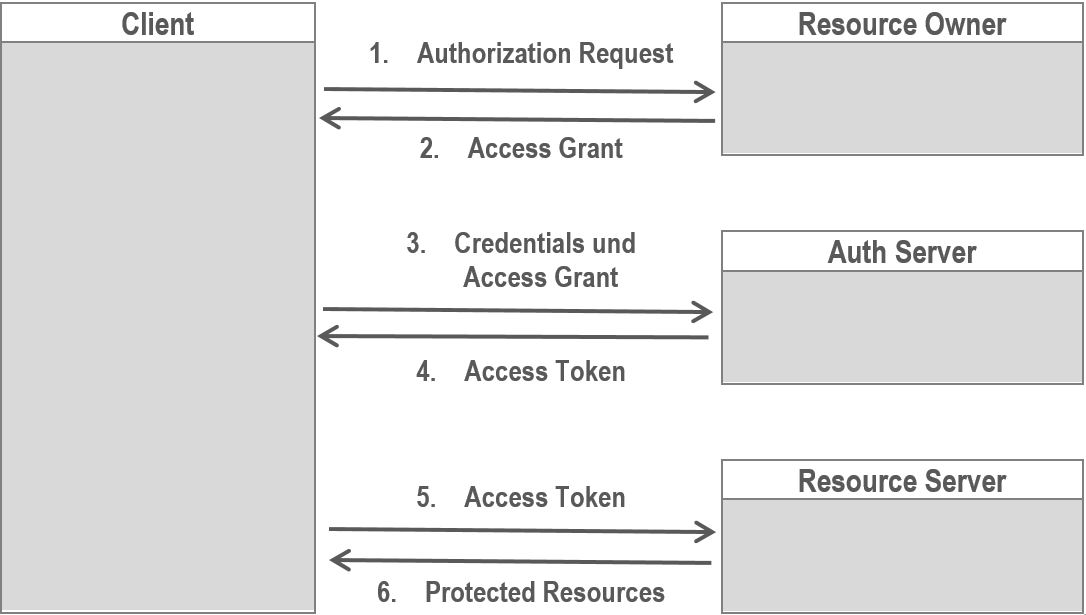
\includegraphics[width=0.8\linewidth]{images/oaut-process2}
		\caption{OAuth Authorization Process (\cite{LeBlanc:2011:SocialApplications}, p.353)}
		\label{fig:oaut-process2}
	\end{figure}
	
	In the first two steps, the Client redirects the User to the Resource Owner, to give the Client permission to access the protected resources. The User is then redirected to the callback location which is included in the original request and adds a verification code which confirms that the Client is entitled to access the requested resource. After the redirection to the callback location, the Client sends a request with the verification code to the Authorization Server. If the request is a success, the Authorization Server replies in step 4 with an access token and eventually a refresh token. With the received access token the Client can know to make signed requests to the resource server and receive protected resources as shown in step 5 and 6 [cf. (\cite{LeBlanc:2011:SocialApplications}, p. 353)]
	
	OpenID Connect and OAuth 2.0 seem very similar, in fact, OpenID Connect is a framework build on top of OAuth 2.0. Together they focus on Authentication and Access Control in a way that is suitable for modern applications. OpenID can verify the identity of an End-User and obtain basic profile information about the user. It uses Claims to communicate information to the End-User [cf. (\cite{Sakimura:2014:OpenIDConnect})]
	
	OpenID Connect performs authentication and determines if the user is already logged on or to log on the user. The result is an authentication token which is returned to the user. A precondition of OpenID Connect is that the client, as well as the user, have to trust the IdP. The functions of the IdP are the same as in OAuth. The reason for that is that the newest version of OpenID is implemented on top of OAuth and extends the authentication process of OAuth  [cf. (\cite{Sakimura:2014:OpenIDConnect}), (\cite{Boyd:2012:GSOAuth}, p.51)]
	
	\begin{figure}[h]
		\centering
		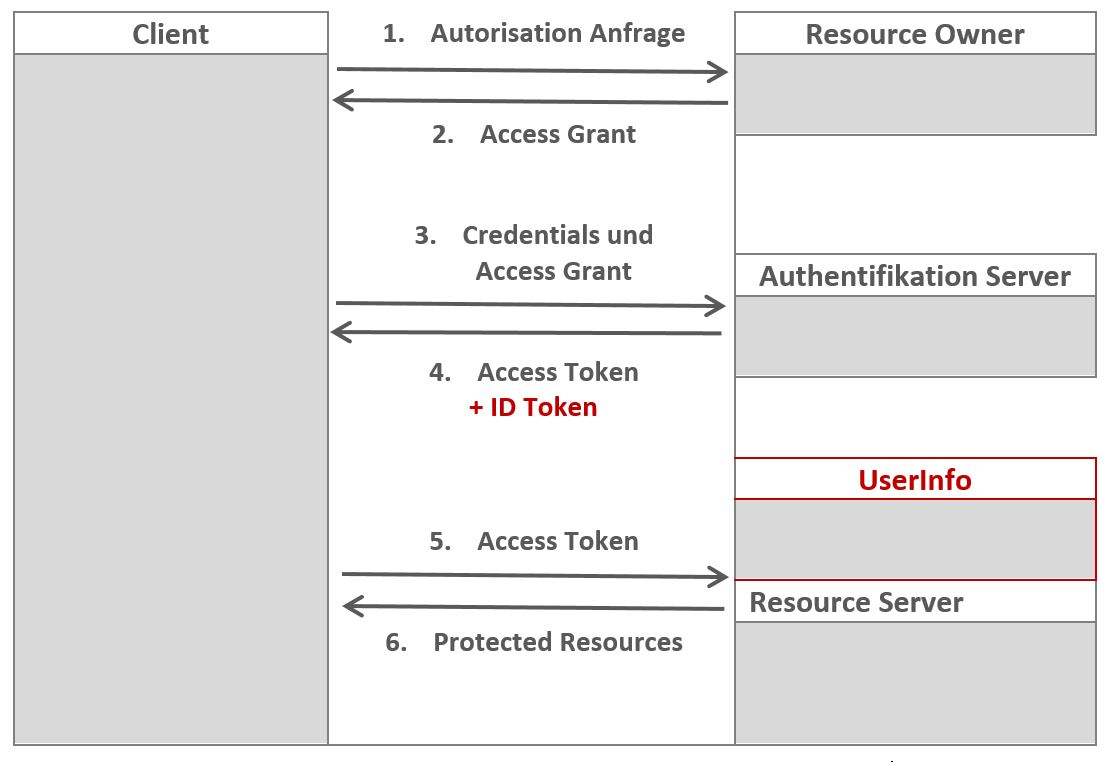
\includegraphics[width=0.8\linewidth]{images/openid-process}
		\caption{OAuth 2.0 and OpenID Connect \cite{Lodderstedt:2014:OpenID}}
		\label{fig:openid-process}
	\end{figure}
	
	
	In figure \ref{fig:openid-process} OAuth 2.0 and OpenID Connect \cite{Lodderstedt:2014:OpenID} the added Element of the OpenID Connect standard is marked with red. In order to implement the OpenID Connect Standard, the Client has to request the scope 'openid'. After the request, the progress is similar to the transitional OAuth authentication process, but when it comes to return of the access token, a additional ID Token is returned. This ID Token holds information about the user and the authentication. The only purpose of the ID Token is to log in the client. The only thin left after this is for the client to verify the ID Token [cf. \cite{Lodderstedt:2014:OpenID}]. 
	
	The ID Token is specified by \cite{Sakimura:2014:OpenIDConnect} as a JWT compared to OAuth were the type of token is irrelevant. The token is signed and has some particular claims. Further individual claims could also be added to the ID token. The ID token has claims that are required for the authentication process. Also, standard claims can be added which are predefined by OpenID Connect. Those claims could also be requested from UserInfo Endpoint shown as an additional endpoint in the figure \ref{fig:openid-process} OAuth 2.0 and OpenID Connect \cite{Lodderstedt:2014:OpenID}. The user info endpoint offers an API where additional user info can be requested [cf. (\cite{Sakimura:2014:OpenIDConnect})].
	
	\cite{Lodderstedt:2014:OpenID} says that OpenID Connect is a contemporary advancement from protocols like SAML. The protocol considers the ongoing development of web services and mobile applications. Furthermore, the implementation of the protocol is quite easy and uses little HTTP requests with minimal cryptographic overhead to accomplish a complete login process [cf. (\cite{Lodderstedt:2014:OpenID})]. 
	
	
	
	
	
	
	\cite{Sakimura:2014:OpenIDConnect} defines three different way authentication can flow:
	
	
	\begin{enumerate}
		\item \textbf{Authorization Code Flow}  - The Authorization Code Flow returns an Authentification Code which can be used to be exchanged for an id\_token or an access\_token. The Authorization Code is used for Clients that can maintain a secret securely between themselves and the Authorization Server. Typically this approach is used for server-to-server communication when no interactive user is present. In this thesis, the focus is on user interaction [cf. (\cite{Sakimura:2014:OpenIDConnect}, p.10)]
		
		To use the Authorization Code Flow according to \cite{Sakimura:2014:OpenIDConnect} the the following request\_type indicates a Authorization Code Flow:
		\begin{itemize}
			\item	code: The response includes an Authorization Code. 
		\end{itemize}
		
		\item \textbf{Implicit Code Flow} - In the Implicit Code Flow the access token and the ID id token are directly returned to the Client. This behavior may expose information to the End-User or anyone who has access to the End-User’s Agent. Tokens are only returned from the Token Endpoint; the Authorization Endpoints is not used. Unlike the Authorization Code Flow where the separate request is used for authorization and authentification, here the Client will receive the access token as a result of the authentification which also means that there is no refresh token.  This flow is used for Clients who are implemented in a browser using scripting language [cf. (\cite{Sakimura:2014:OpenIDConnect}, p.20), (\cite{Hardt:2012:OAuth2})]
		
		According to \cite{Sakimura:2014:OpenIDConnect}, the following request\_types indicate an Implicit Code Flow:
		\begin{itemize}
			\item	id\_token: The response must include the parameter id\_token. The response does not include an Authorization Code, Access Token, or Access Token Type. 
			\item  id\_token token: The response includes an Access Token, an Access Token Type and an id\_token.
		\end{itemize}
		
		\item \textbf{Hybrid Code Flow} - In the hybrid code flow, tokens are returned from the Authorization Endpoint, and others are returned from the Token Endpoint. The Token Server will return not only the id token but also the code. The Client then has to use the code in order to gain the access token through a back channel call which means there is an additional round trip compared to the Implicit Code Flow. Using the code to receive the access token should minimize the risk of exposing the access token [cf. (\cite{Sakimura:2014:OpenIDConnect})].
		To use the Hybrid Code Flow according to de \cite{Sakimura:2014:OpenIDConnect} put forward that the following request\_types indicate a Hybrid Code Flow:
		\begin{itemize}
			\item	code id\_token: The response includes an Authorization Code and an id\_token.
			\item  code id\_token token: The response includes an Authorization Code, an Access Token, an Access Token Type and an id\_token. 
		\end{itemize} 
		
	\end{enumerate}
	
	Both OpenID and SAML SSO solution involve different layers of communication and exchange credentials using HTTP redirection and Javascript which leads to vulnerabilities. Vulnerabilities include Cross-Site Request Forgery and Cross Site Scripting. 
	

	The authentication process for SSO solution includes redirects which can be exploited by attackers. As the SP redirects the User to the IdP, an attacker could intervene and send the user to a fake IdP. If the user does not recognize to swap from the real IdP to the fake IDP, the attacker ends up with the user's credentials. This problem is called a malicious IdP, also known as “phishing” and a very well-known attack against SSO. Another problem that a federation single sign-on system could be facing is a malicious RP or SP.After a User successfully authenticates on the IdP site, he is redirected back to the SP with a link. An attacker obtains a link with methods like sniffing and uses the link to get logged into the SP as the User [cf. (\cite{Xu:2015:SPSSO})].
	
	TODO:  comparision SAML and OAUTH OPENID

\chapterend